\chapter{Описание программной реализации}
\label{chapter4}

В ходе написания диссертации мы~пришли к~задаче сетевого планирования с~нечёткими временными оценками, описанной в~главе~\ref{chapter3}. В~ней было показано, что эта задача может решаться как с~помощью методов математического программирования, так~и алгоритмически. В~данной главе строится и~описывается программный модуль, позволяющий выполнять сетевой анализ проекта в нечётких условиях с использованием двухточечных и $\alpha$-уровневых вычислений и формировать отчёт о решении в формате Microsoft Excel с наглядным представлением критического пути проекта и рассчитанными модифицированными сроками наступления событий. Особенностью описываемого модуля является то, что он не использует никаких специализированных средств и третьесторонних библиотек для представления нечётких чисел и выполнения операций над ними, как это делается, например, в~\cite{Gallyamov, Kruglov_Balashov, Koroteev_Fuzzy_Arithmetics}, а обходится только стандартными вычислениями с применением действительных переменных. Это преимущество позволило в большей степени сфокусироваться на разработке и тестировании алгоритмов решения чётких $\alpha$-уровневых задач, а также логических модулей, повышающих удобство работы с программным продуктом.

\newpage
\section{Календарно-сетевое планирование в сфере разработки программного обеспечения} 
\label{chapter4_1}
Перспективность данного направления исследований заключается в преимуществах теории нечётких множеств при обработке нечётких данных, которыми изобилует реальная практика разработки ПО в сфере аутсорсинга. Действительно, характерными чертами процесса проектирования и разработки программного обеспечения являются:
\begin{itemize}
  \item относительная уникальность разрабатываемого проекта~--- у некоторых участников может быть опыт участия в схожих проектах, однако он нивелируется тем, что остальная часть команды обычно впервые сталкивается с конкретной задачей автоматизации в некоторой предметной области;
  \item частое отсутствие полных требований к программному продукту либо необходимых для разработки ресурсов (согласованные и утверждённые дизайны, переводы и т.д.);
  \item разный уровень подготовки членов команды разработчиков;
  \item возможность изменения списка работ на поздних стадиях разработки~--- либо увеличение списка требований к продукту, либо его сокращение с целью ускорить разработку и приурочить выпуск готового продукта к некоторому событию;
  \item бюрократическая составляющая~--- затягивание сроков разработки из-за проблем в согласовании изменений или списка работ;
\end{itemize}

В связи с~этим в настоящее время применяемые при планировании разработки ПО методы в основном являются неформальными и базируются на использовании мнений нескольких экспертов. Эксперты, производящие первоначальную оценку проекта, обычно знают о вышеперечисленных потенциальных рисках и~потому стараются учесть все риски в самих временных оценках. Чаще всего применяется вариант интервальной неопределённости, т.\,н. <<вилка>>~--- оценка наиболее пессимистичного и наиболее оптимистичного вариантов разработки. Однако у этого варианта есть несколько существенных недостатков:
\begin{itemize}
  \item обычно заказчики ориентируются на нижнюю границу оценки и не уточняют список потенциальных факторов риска, которые приводят к достижению верхней границы интервала, при этом вынуждая руководителя проекта надавливать на экспертов с целью получения более оптимистичной и точной оценки;
  \item существует негласное правило <<умножения на три>>, которое применяется руководителем проекта при анализе оценок, полученных от экспертов: для каждого этапа проекта из полученных оценок выбирается самая пессимистичная и утраивается~--- в результате неопределённость учитывается дважды; 
  \item эксперт, коим обычно является инженер-программист, исходит из своего опыта и оценки собственной производительности, поэтому оценка может оказаться чрезмерно персонализированной~--- другой исполнитель задания просто не успеет выполнить запланированные работы в срок.
\end{itemize}

В связи с этим логичным выглядит получение оценок в виде нечётких треугольных чисел, поскольку эксперт на основании своего опыта может оценить, сколько времени обычно занимает некоторый этап разработки, и сколько времени он занимал в наилучшем и наихудшем случаях. Учитывая общую склонность инженеров-программистов к пессимистическому оцениванию времени разработки, оценки обычно получаются асимметричными. Применение к оценкам преобразования L позволяет получить модифицированные значения оценок, носители которых могут быть в дальнейшем интерпретированы как нечёткие интервалы, а тип (LL или RR)~--- как степень пессимизма или оптимизма. 

Рассмотрим следующий случай. В фирму по разработке программного обеспечения обращается заказчик с просьбой оценить срок и примерную стоимость реализации комплексного решения~--- веб-портала и двух мобильных приложений под наиболее популярные платформы~--- приуроченного к празднованию круглой даты одного из государственных праздников. Для оценки продолжительности проекта собирается команда экспертов, состоящая из руководителя проекта, графического дизайнера, разработчика серверных приложений и двух разработчиков мобильных приложений. Требуется предоставить заказчику <<вилку>> по времени и указать возможные факторы риска незавершения проекта в срок.

В~cтандартный процесс оценивания проекта, состоящий из этапов идентификации операций, построения их взаимосвязей, оценки их продолжительностей и расчёта общего времени проекта, вносятся некоторые изменения. После идентификации операций строится т.\,н. вершинный граф проекта~\cite{Eddous, Taha_Operation_Research}, в котором операции представляются вершинами графа, а дугами показаны их зависимости друг от друга. Построение вершинного графа занимает гораздо меньшее время ввиду отсутствия в нём проблемы фиктивных стрелок, однако для решения задачи планирования лучше подходит стрелочный граф~--- именно на такое представление проекта рассчитаны методы, описанные в главе~\ref{chapter3}. Решить это противоречие позволяет преобразование вершинного графа в стрелочный~\cite{VSU-5y}. В~основу алгоритма преобразования положены следующие правила построения стрелочного графа, описанные в~\cite{Eddous, Taha_Operation_Research}.
\begin{enumerate}
\label{Taha:ConversionRules}
  \item Каждый процесс в проекте представляется только одной дугой.
  \item Каждый процесс идентифицируется двумя концевыми узлами.
  \item Для поддержкания правильных отношений предшествования при включении в сеть любого процесса, необходимо идентифицировать, какой процесс непосредственно предшествует текущему, какой должен выполняться после заверения текущего и какой выполняется параллельно с текущим. В результате идентификации соседних процессов принимается решение о том, требуется ли включить в сеть фиктивные операции для правильного отображения последовательности выполнения задач.
\end{enumerate}

Ниже описана последовательность шагов по преобразованию вершинного графа в стрелочный~\cite{VSU-5y}. $d_i^-$ обозначает число входящих в вершину $v_i$ дуг, $d_i^+$~--- число исходящих, а сумма этих значений равна степени вершины $d_i=d_i^-+d_i^+$.
\begin{enumerate}
\label{ConversionAlgo}
	\item Топологическая сортировка исходного вершинного графа для определения порядка следования операций и начальных вершин графа.
	\item \label{question:veer} Создание начального узла стрелочного графа и исходящих из него дуг-операций. Для этого из исходного вершинного графа $ G_v = (V_v,E_v)$ выбираются те вершины, у которых нет входящих в них стрелок, т.е. все $v_i \in V_v: d_{v_i}^-=0$. Для этих $N$ операций в новом стрелочном графе создаётся $N+1$ вершина, одна из которых будет общей начальной вершиной для всех стрелок. В итоге получается <<веер>> из вершин, изображённый на рис.~\ref{fig:graph-transform-source}.
	\begin{figure}[h!]
		\centering
		{
			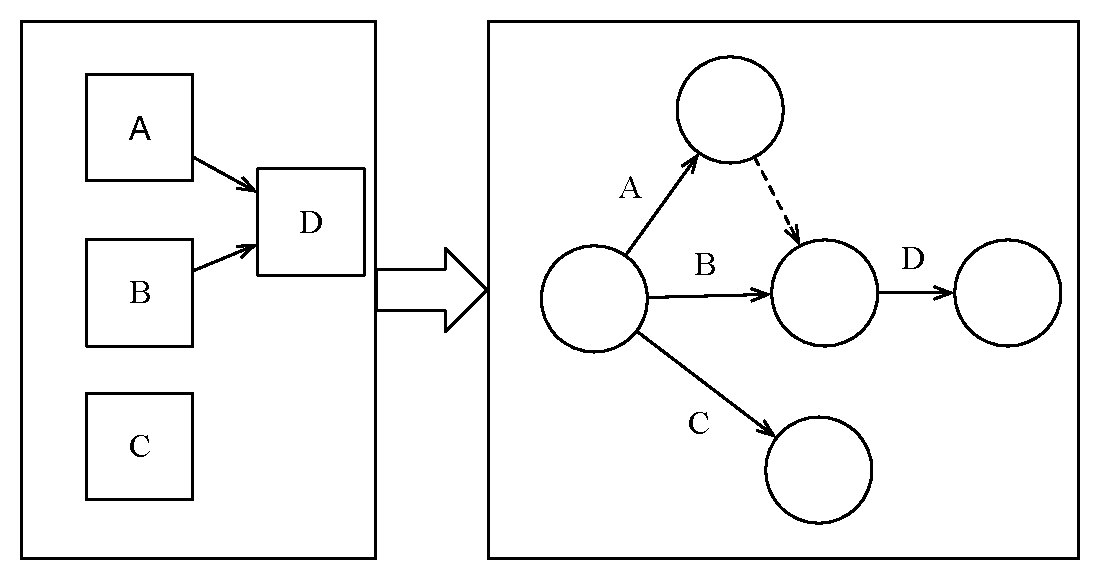
\includegraphics[width=0.9\textwidth]{graph-transform-source}
		}
		\caption{Преобразование начальных операций проекта}
		\label{fig:graph-transform-source}
	\end{figure}
	\item Поочередное добавление оставшихся операций. Для операций, которые ещё не были добавлены в граф, возможны следующие варианты:
	\begin{enumerate}
		\item Добавляемой операции непосредственно предшествует ровно одна операция. В этом случае конечная вершина стрелки, соответствующей непосредственно предшествующей операции, является начальной для новой стрелки. Пример изображён на рис.~\ref{fig:graph-transform-middle}~--- операции $I$ непосредственно предшествует только одна операция  $G$.
		\begin{figure}[h!]
			\centering
			{
				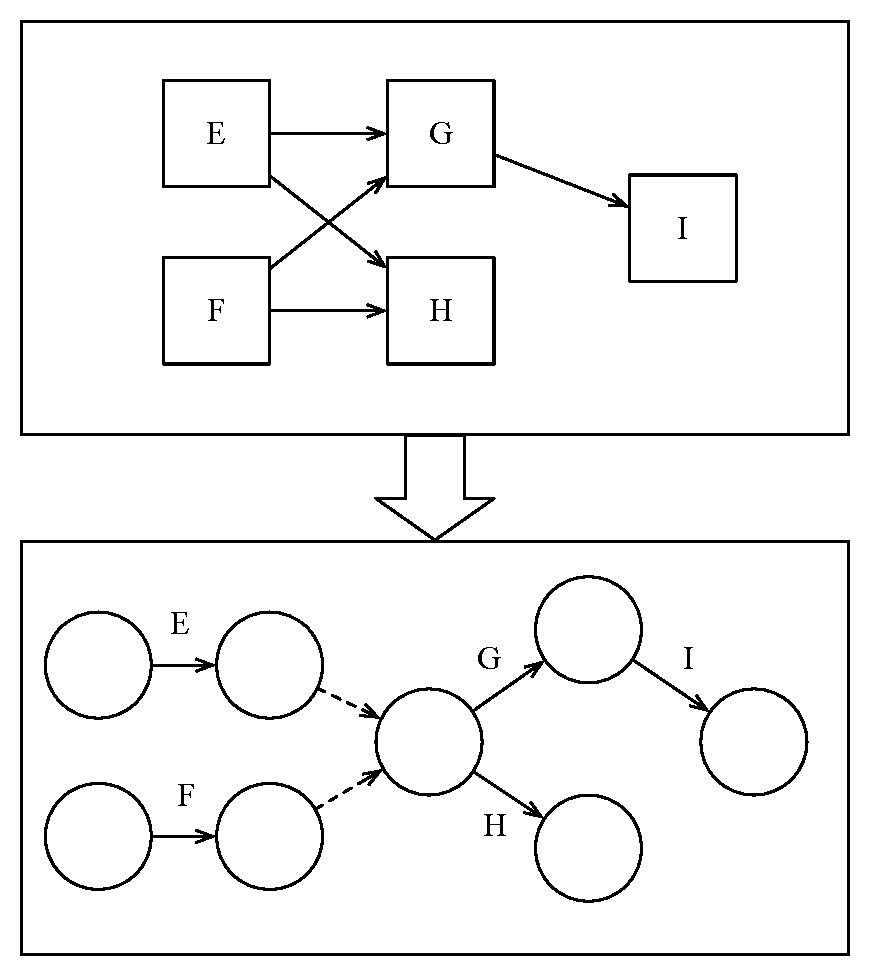
\includegraphics[width=0.75\textwidth]{graph-transform-middle}
			}
			\caption{Дальнейшее добавление операций}
			\label{fig:graph-transform-middle}
		\end{figure}
		\item Добавляемой операции непосредственно предшествует несколько операций. В этом случае в вершинном графе ищутся другие операции, которые ещё не были добавлены в новый граф, и у которых тот же набор непосредственно предшествующих операций. Если таких операций оказалось несколько, то выполняются действия, аналогичные описанным в~п.~\ref{question:veer}, и добавляются фиктивные дуги, соединяющие конечные вершины предшествующих операций и начальную вершину "веера". На рис.~\ref{fig:graph-transform-middle} у вершин $G$ и $H$ как раз одинаковые непосредственно предшествующие вершины $E$ и $F$. Иначе создаётся единственная дуга, начало которой соединяется фиктивными дугами с концами непосредственно предшествующих вершин.
	\end{enumerate}
	\item Соединение концов завершающих дуг в одной вершине. Для этого в созданном стрелочном графе выбираются все вершины $v_i \in V$: $d_{v_i}^+=0$, и создаётся единственная конечная вершина. Все дуги, входящие в вершины $v_i$, перенаправляются на новую вершину, а старые конечные вершины удаляются. Пример такого преобразования можно увидеть на рис.~\ref{fig:graph-transform-sink}
	\begin{figure}[h!]
		\centering
		{
			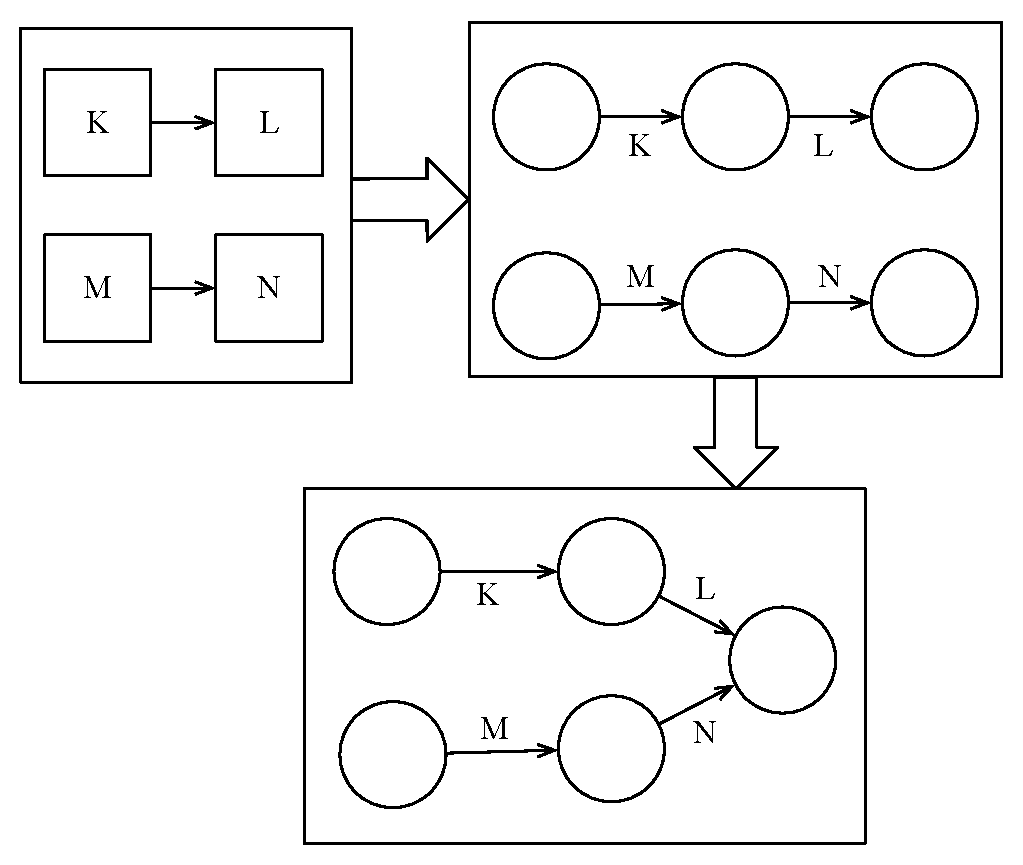
\includegraphics[width=0.9\textwidth]{graph-transform-sink}
		}
		\caption{Соединение конечных дуг в одной вершине}
		\label{fig:graph-transform-sink}
	\end{figure}
	\item Упрощение графа с помощью удаления фиктивных дуг. На последнем этапе происходит уменьшение числа дуг в соответствие с правилами, описанными на стр.~\pageref{Taha:ConversionRules}. В построенном стрелочном графе $G_S$ выбираются все фиктивные дуги $e_{F_i}=\left(v_{S_i}; v_{E_i}\right)$; затем для каждой $e_{F_i}$ происходит проверка, не используется ли она для обозначения параллельно выполняющихся процессов. Проверяются следующие условия:
	\begin{itemize}
		\item из начальной вершины $v_{S_i}$ дуги $e_{F_i}$ не выходит никаких других дуг, кроме самой $e_{F_i}$;
		\item $V_P(v_{S_i}) \bigcap V_P(v_{E_i}) = \varnothing $ и $V_S(v_{S_i}) \bigcap V_S(v_{E_i}) = \varnothing$, где $V_P(v_i), V_S(v_i)$~--- множества вершин, непосредственно предшествующих вершине $v_i$ и непосредственно следующих за $v_i$ соответственно.
	\end{itemize}
	 Если оба этих условия выполняются, то можно исключить проверенную дугу из графа, объединяя её начальную и конечную вершины.
\end{enumerate}

После построения сетевого графика, эксперты-разработчики формулируют интервальные оценки $\left[ x_i^L, x_i^R \right]$ для всех операций проекта, но при этом их дополнительно просят указать наиболее возможный, с их точки зрения, срок выполнения операции $m_i$. Вместе эти три параметра используются для формирования нечёткой треугольной оценки $\tau_i=\left \langle x_i^L, m_i, x_i^R \right \rangle = \left \langle m_i, m-x_i^L, x_i^R-m \right \rangle$. Полученные нечёткие оценки $\tau_i$ в дальнейшем будут использованы для расчёта общего времени выполнения проекта и поиска критического пути.

Критический путь и~время выполнения проекта находятся с~помощью модификации классического алгоритма Дейкстры. Возможны два варианта поиска критического пути: двухточечный, когда расчёты выполняются дважды~--- при $\alpha=0$ и $\alpha=1$, и $\alpha$-уровневый, при котором задаётся число уровней поиска $q$, и~алгоритм для чёткого случая выполняется $q$ раз на~различных $\alpha$-уровнях, расстояние между которыми равно $\displaystyle \frac{1}{q}$. В~первом случае модифицированное нечёткое время выполнения восстанавливается согласно~\eqref{eq:isomorphic-field}, а во втором на выходе получается нечёткая величина с дискретной функцией принадлежности, которую также в большинстве случаев удаётся интерполировать линейной зависимостью.

Найденные общее нечёткое время выполнения проекта и критические операции могут быть представлены заказчику как <<вилка>> и потенциально рискованные операции соответственно.

Перейдём к~описанию программного средства, призванного автоматизировать процесс получения нечёткой временной оценки проекта и~соответствующий ей критический путь.


\section{Программное обеспечение} 
\label{chapter4_2}
\textit{Средства разработки}. В качестве средства разработки применяется интегрированная среда Microsoft Visual Studio 2010. Эта среда разработки поддерживает компонентную технологию, позволяет легко создавать собственные компоненты и интегрироваться с внешними модулями ПО и офисными пакетами.

\textit{Требования к аппаратному и программному обеспечению}. Для нормального функционирования программы необходимы следующие программные и технические средства:
\begin{itemize}
  \item Intel-совместимый процессор с тактовой частотой не менее 1 ГГц;
  \item объём оперативной памяти~--- 1 ГБ и более;
  \item свободное место на жёстком диске~--- 100 МБ и более;
  \item операционная система~--- Windows 7 и выше;
  \item предустановленная среда выполнения .NET Framework Client Profile версии не ниже 4.0;
  \item предустановленный пакет визуализации Graphviz версии не ниже 2.28;
  \item предустановленный офисный пакет Microsoft Office версии не ниже 14 (Office 2010).
\end{itemize}

\textit{Условия применения программы.} Разработанная программа решает научно-исследовательскую и прикладную задачи. Программа распространяется свободно и без каких-либо ограничений и гарантий.

\subsection{Программный модуль CSBusinessGraph}

\subsubsection*{Назначение программы}

Разработанная программа предназначена для проведения вычислительного эксперимента по сетевому анализу проектов в условиях нечёткой неопределённости, цель которого заключалась в апробации описанных в~главе~\ref{chapter2} двухточечных вычислений и сравнении их результатов с результатами $\alpha$-уровневых вычислений.

\subsubsection*{Интерфейс пользователя}
Программа имеет интуитивно понятный интерфейс, представленный на рис.~\ref{fig:app-main}. На нижней панели расположены элементы управления представлением~--- кнопки и ползунок, позволяющие изменять масштаб. Для создания нового проекта необходимо выбрать пункт меню <<File~--- New Project>> (Файл~--- Новый проект). Также возможна загрузка ранее созданного проекта для редактирования. Для этого необходимо выбрать пункт меню <<File~--- Open Existing Project>> (Файл~--- Открыть существующий проект), после чего будет показан диалог открытия файла 
\begin{figure}[h!]
  \centering
  {
    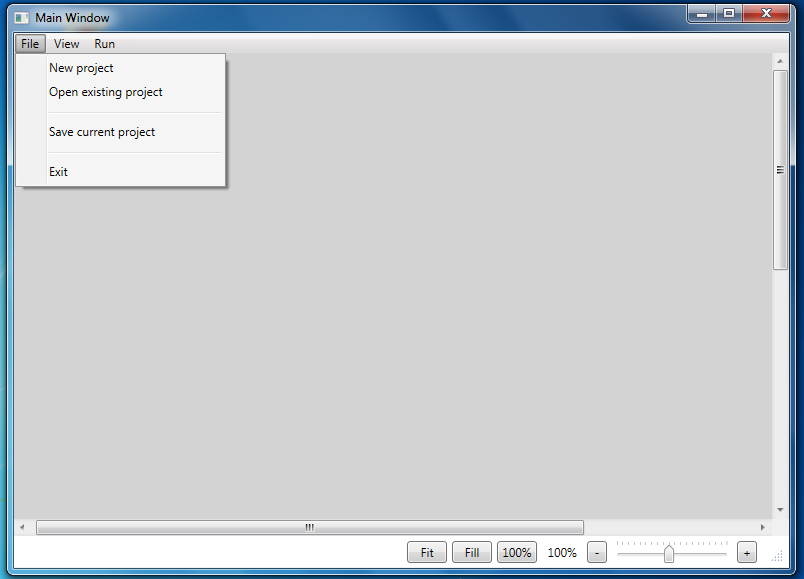
\includegraphics[width=0.85\textwidth]{app-main.png}
  }
  \caption{Главное окно приложения на старте}
  \label{fig:app-main}
\end{figure}

Вначале создаются операции путём вызова контекстного меню (рис.~\ref{fig:app-sample-graph}) и нажатия на опцию <<Create Node>> (Создать узел). При этом появляется окно для ввода и редактирования данных операции, представленное на рис.~\ref{fig:app-edit-window}. Это~же окно можно вызвать, выделив вершину графа и~нажав пункт меню <<View>> (Просмотр). Создание дуги выполняется с помощью механизма <<drag-and-drop>>: левая кнопка мыши нажимается в одной из двух точек узла, называемых точками сопряжения, и отпускается после перетаскивания курсора на вершине, в которую должна входить дуга. 

\begin{figure}[b!]
  \centering
  {
    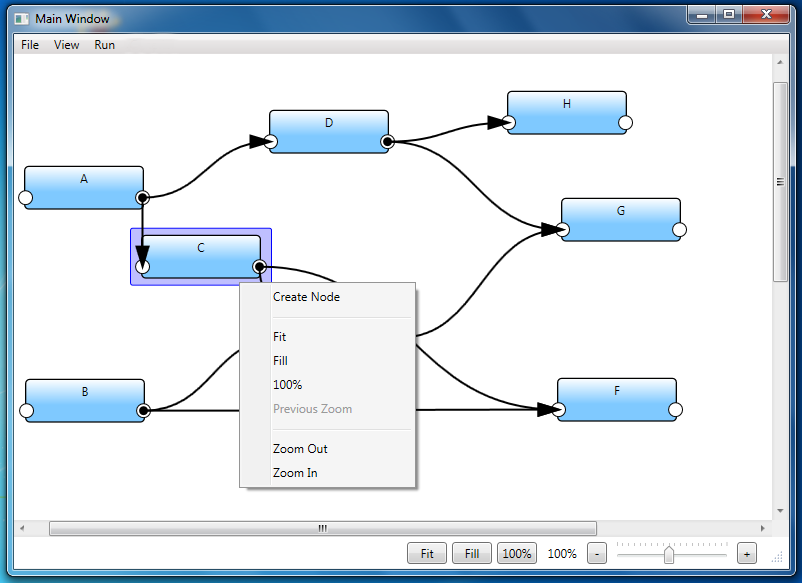
\includegraphics[width=0.85\textwidth]{app-sample-graph.png}
  }
  \caption{Вызов контекстного меню}
  \label{fig:app-sample-graph}
\end{figure}

\begin{figure}[h!]
  \centering
  {
    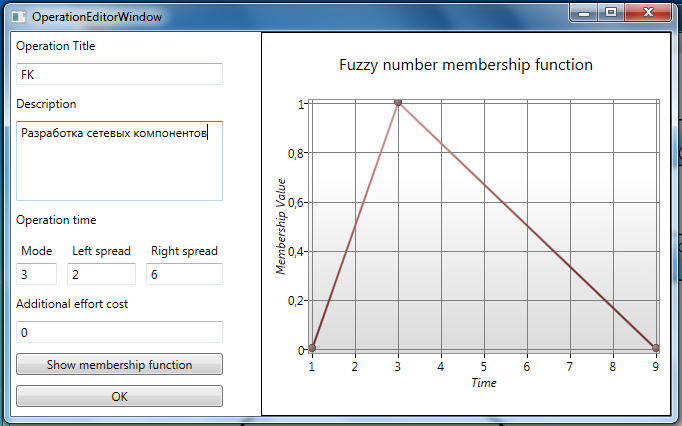
\includegraphics[width=0.9\textwidth]{app-edit-window.png}
  }
  \caption{Окно редактирования характеристик операции}
  \label{fig:app-edit-window}
\end{figure}

Удалить существующую вершину или дугу можно, щёлкнув по всплывающей кнопке в виде ножниц, которя появляется, если задержать над дугой/вершиной курсор мыши (рис.~\ref{fig:app-scissors-button}). 
\begin{figure}[h!]
  \centering
  {
    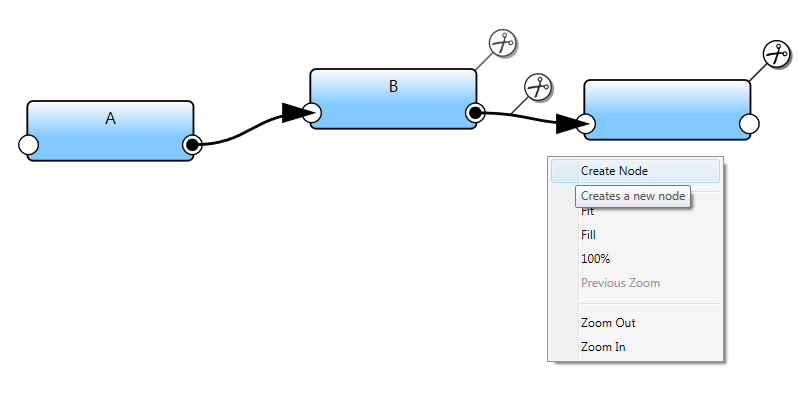
\includegraphics[width=0.8\textwidth]{app-scissors-button.png}
  }
  \caption{Всплывающие кнопки удаления элементов графа}
  \label{fig:app-scissors-button}
\end{figure}

Пункт меню <<Run>> (Запустить) показывает окно, в котором можно выбрать используемое в процессе анализа значение $\lambda$ из списка предопределённых опций (середина отрезка, центр тяжести, оптимум сохранения информации). После выбора пользователем значения $\lambda$, приложение запускает процедуру анализа. По её окончании показывается диалог, позволяющий выбрать место сохранения отчёта в формате Microsoft Excel.

Для выхода из приложения необходимо выбрать пункт меню <<File~--- Exit>> (Файл~--- Выйти) или нажать на стандартную кнопку закрытия окна в правом верхнем углу.

\subsubsection*{Функциональные возможности программы}
Программа имеет следующие функциональные возможности:
\begin{itemize}
  \item создание модели проекта в виде вершинного графа в ручном режиме или импорт существующей модели из XML-файла;
  \item поддержка модели проекта в согласованном состоянии~--- проверка отсутствия циклов в графе и наличие только одной компоненты связности;
  \item редактирование временных оценок выполнения операций, выраженных в~виде треугольных чисел, c~помощью изменения параметров нечёткго числа;
  \item графическое представление функций принадлежности для~временных оценок;
  \item автоматическое преобразование вершинного графа в~стрелочный;
  \item выбор пользователем используемых при~расчётах значений параметров $\lambda$ преобразования L, соответствующих середине $\alpha$-сечения, проекции центра тяжести или оптимальному в смысле сохранения экспертной информации значению;
  \item реализация механизма расчёта критического пути на~основе $\alpha$-уровневых и~двухточечных вычислений;
  \item экспорт отчёта о~решении задачи в~формат Microsoft Excel с~формированием графиков для модифицированных нечётких оценок, общего времени выполнения проекта и~построением преобразованного стрелочного графа c~выделением критических операций.
\end{itemize}

\subsubsection*{Реализация}

\textit{Структура данных}

Входными данными приложения является либо результаты пользовательского ввода, либо документ с описанием структуры проекта и временных оценок. Поскольку моделью проекта является разреженный вершинный граф, то для его хранения в памяти и на диске выбрана структура в виде списков смежности, в которой для каждой вершины указывается список идентификаторов связанных с ней вершин, а также кортеж из трёх действительных чисел, формирующих нечёткую оценку веса вершины. На диске модель проекта хранится в формате XML, что позволяет легко редактировать её.

Выходные данные агрегируются в формат Microsoft Excel и состоят из следующих частей:
\begin{itemize}
  \item две таблицы, соответствующие значениям $\alpha=0$ и $\alpha=1$ и содержащие рассчитанные для каждой операции проекта наиболее ранние и наиболее поздние сроки наступления её начального и конечного событий, а также полные резервы времени. Операции, принадлежащие критическому пути, выделены цветом;
  \item изображение полученного в результате преобразования стрелочного графа с нанесённым на него критическим путём;
  \item графики функций принадлежности для модифицированных нечётких продолжительностей операций.
\end{itemize}

\textit{Логическая структура программы}

Программа состоит из нескольких модулей, организованных в соответствие с шаблоном <<модель--представление--модель представления>>~\cite{NetworkView_CodeProject}. Схема взаимодействия между модулями программы показана на рис.~\ref{fig:app-architecture}.
\begin{figure}[t!]
  \centering
  {
    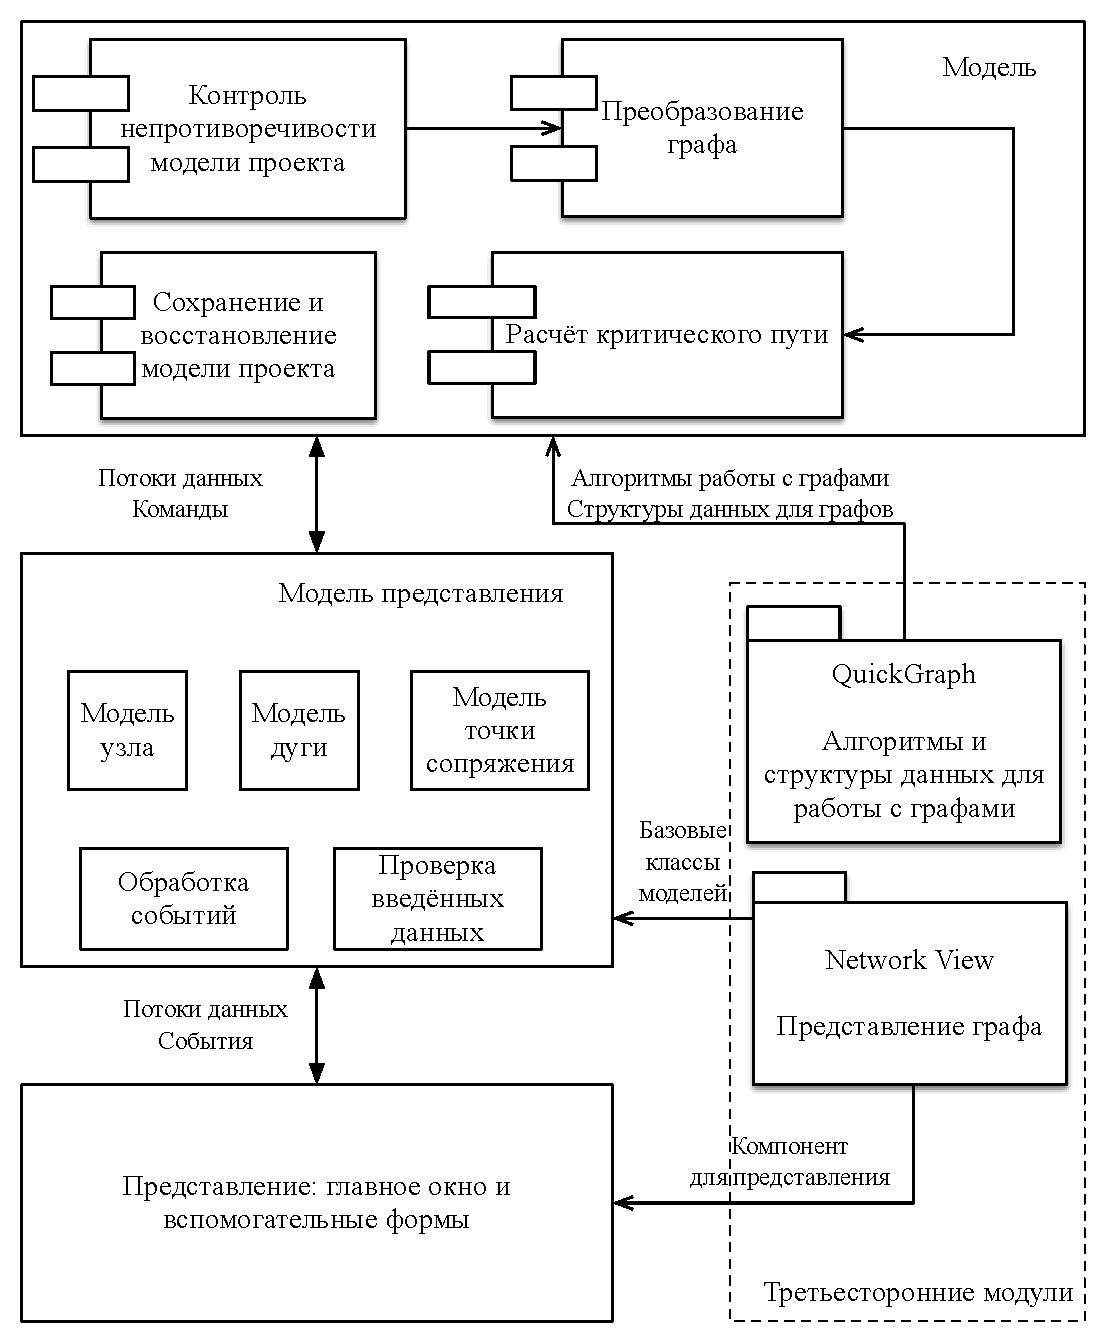
\includegraphics[width=0.7\textwidth]{app-architecture}
  }
  \caption{Взаимодействие между модулями приложения}
  \label{fig:app-architecture}
\end{figure}

Как видно из рис.~\ref{fig:app-architecture}, в~программе были использованы третьесторонние компоненты, позволившие сократить общее время разработки и упростить тестирование~--- библиотека для~работы с~графами QuickGraph~\cite{QuickGraph_Codeplex, QuickGraph_CodeProject} и~компонент для~визуального представления и~редактирования графа NetworkView~\cite{NetworkView_CodeProject}.

В программном модуле реализован алгоритм автоматического преобразования вершинного графа в стрелочный, описанный на стр.~\pageref{ConversionAlgo}. Автоматический контроль согласованности выполняется с~помощью алгоритма поиска в~глубину при~добавлении каждой новой вершины.

\subsubsection*{Тестирование приложения}

Результаты тестирования приложения приведены в таблице~\ref{t:app-testing}.

\begin{center}
\begin{longtable}[h!]{|p{6.45cm}|p{0.55\linewidth}|}
\caption{Результаты тестирования приложения} \label{t:app-testing}\\
    \hline
      \textbf{Тест} & \textbf{Результат теста} \tabularnewline \hline
	\endfirsthead
	\caption*{Продолжение таблицы~\ref{t:app-testing}} \\
    \hline
	  \textbf{Тест} & \textbf{Результат теста} \tabularnewline \hline
	\endhead
	\hline
		Проверка доступности пунктов меню и кнопок на форме приложения & Доступны пункты меню \\ \hline
        Выбор пункта меню <<File~--- New Project>> (Файл~--- Новый проект) & Создаётся новый проект и показывается пустая рабочая область окна \\ \hline
		Выбор пункта меню <<File~--- Open existing Project>> (Файл~--- Открыть существующий проект) & Показывается диалог выбора файла с расширением *.csbgproj. Выбор файла и нажатие на кнопку <<Открыть>> приводит к загрузке проекта и его отображению на экране \\ \hline
        Выбор пункта меню <<File~--- Save Current Project>> (Файл~--- Сохранить текущий проект) & Показывается диалог сохранения файла с расширением *.csbgproj. По нажании на кнопку <<Сохранить>> создаётся файл проекта с указанным именем в указанной папке \\ \hline
		Вызов контекстного меню и выбор опции <<Create Node>> (Создать узел) & Создаётся новая вершина графа и открывается окно редактирования параметров операции. При не полностью введённых данных программа выдаёт предупреждение. При нажатии на кнопку <<Show membership function>> (Показать функцию принадлежности) строится график функции принадлежности треугольного числа с указанными параметрами. Кнопка <<OK>> позволяет закончить редактирование и продолжить работу с проектом \\ \hline
		Выделение вершины графа и выбор пункта меню <<View>> (Просмотр) & Открывается окно редактирования параметров операции\\ \hline
		Нажатие левой кнопки мыши на точке сопряжения, перетаскивание курсора мыши при зажатой левой кнопке и отпускание мыши на целевой вершине & Создаётся дуга графа между двумя вершинами \\ \hline
		Создание дуги из одной вершины в другую при наличии обратной дуги & Приложение выдаёт предупреждение о невозможности операции ввиду нарушения свойства ацикличности и не создаёт дугу \\ \hline
		Нажатие кнопки с изображением ножниц, связанной с дугой & Удаление дуги графа \\ \hline
		Нажатие кнопки с изображением ножниц, связанной с вершиной & Удаление вершины графа и всех связанных с ней дуг~--- входящих и исходящих \\ \hline
		Выбор пункта меню <<Run>> & Проверка числа компонент связности графа~--- если их больше одной, то приложение выдаёт предупреждение о невозможности запуска анализа. Иначе предлагается выбор значения параметра преобразования $L$. После выбора пользователем предпочитаемого значения параметра запускается анализ проекта, по окончании которого приложение выводит диалог сохранения отчёта в формате Microsoft Excel \\ \hline
		Нажатие стандартной кнопки <<Закрыть окно>> или выбор пункта меню <<File~--- Exit>> (Файл~--- Выход) & Завершение работы приложения \\
    \hline
\end{longtable}
\end{center}

\newpage
\section*{Выводы по четвёртой главе:} 
\label{chapter4_3}
\begin{enumerate}
  \item Рассматривается прикладная задача~--- оценка продолжительности выполнения проекта по разработке программного продукта и выделение потенциальных рисков. С помощью алгоритма преобразования вершинного графа в стрелочный модель проекта в виде вершинного графа, удобная для экспертов, преобразовывается в модель, подходящую для автоматизации анализа. А с помощью алгоритма поиска критического пути в проекте с нечёткими оценками находятся общее нечёткое время выполнения и критические операции.
  \item Разработан программный комплекс, позволяющий выполнять автоматизированный сетевой анализ проекта с нечёткими временными оценками и включающий в себя проблемно-ориентированную составляющую для решения задачи оценки рисков и времени выполнения проекта в сфере разработки программного обеспечения. Программный модуль не использует никаких специализированных средств и третьесторонних библиотек для представления нечётких чисел и выполнения операций над ними и выполняет все вычисления только с использованием действительных переменных.
\end{enumerate}